%TODO: refer to grid convolutions as discrete (?)


\chapter{Introduction}
\label{chap:intro}

Many cellular processes rely on proteins, which facilitate these processes via their interactions with one another and with small molecules within the cell~\cite{scheeffink2003}.
%TODO: mention protein interaction networks?
Understanding protein interactions is key to disease and pharmaceutical research, as well as our understanding of basic cellular biology~\cite{fauman2003, altman2003}.
Proteins normally interact via an \textit{interface}, a localized region of the protein with special properties.

Experimentally identifying the interface between two proteins is a time consuming and expensive process which involves crystallization of the protein complex and imaging via x-ray crystallography or nuclear magnetic resonance~\cite{bijelic2017, ilarisavino2017, wang2017}.
In contrast, computational methods are faster, cheaper, and complement wet lab experiments by identifying the most relevant and worthwhile experiments to attempt in vivo.

This thesis presents a novel computational method to predict the interface between a pair of interacting proteins.
The method is inspired by the success of convolutional neural networks in image processing~\cite{gu2015, lecun2010}, but adapts the ideas to this problem domain.
Proteins are represented as graphs and fed into a pairwise convolutional neural network with specialized convolution operations.
The network makes predictions on pairs of amino acid residues of the likelihood that they constitute a part of the interface. 
This method outperforms the existing state-of-the-art approach based on a support vector machine with pairwise kernels~\cite{minhas2014}.

%TODO: Update when done
The rest of this thesis is organized as follows.
The remainder of the introduction presents a primer on proteins and their interfaces. 
Chapter \ref{chap:relatedwork} reviews prior work in interface prediction.
Chapter \ref{chap:neuralnetworks} introduces neural networks and specifically convolutional neural networks.
Chapter \ref{chap:methods} describes the graph convolutional networks and the deep learning architecture used in this thesis.
Chapter \ref{chap:experiments} describes the data set and experiments performed and presents findings. 
Chapter \ref{chap:future} lays out potential avenues of research which build upon the findings in this thesis. 
Appendix \ref{appendix:features} contains details pertaining to the features computed for each amino acid residue, and Appendix \ref{appendix:tools} describes the software and tools that were created and/or used for this research.

\section{Proteins}

DNA is rightly considered the "blueprint for life," which begs the question, what is built from those blueprints?
The answer is, in many cases, the information contained in DNA is used to synthesize proteins.
Proteins are composed of amino acids linked in a chain and held together by covalent bonds.
Amino acids are organic compounds consisting of a central \textit{$\alpha$-carbon} atom, which binds to an \textit{amine group} ($\mathrm{NH_2}$), a \textit{carboxyl group} ($\mathrm{COOH}$), a single hydrogen atom, and a \textit{side chain}, in a tetrahedral geometry.
There are 21 unique amino acids encoded in eukaryotic DNA, each of which has a distinct side chain that gives rise to structural and electro-chemical properties.
Figure \ref{fig:aminoacids} depicts the different amino acids.

\begin{figure}
	\centering
	%\begin{center}
	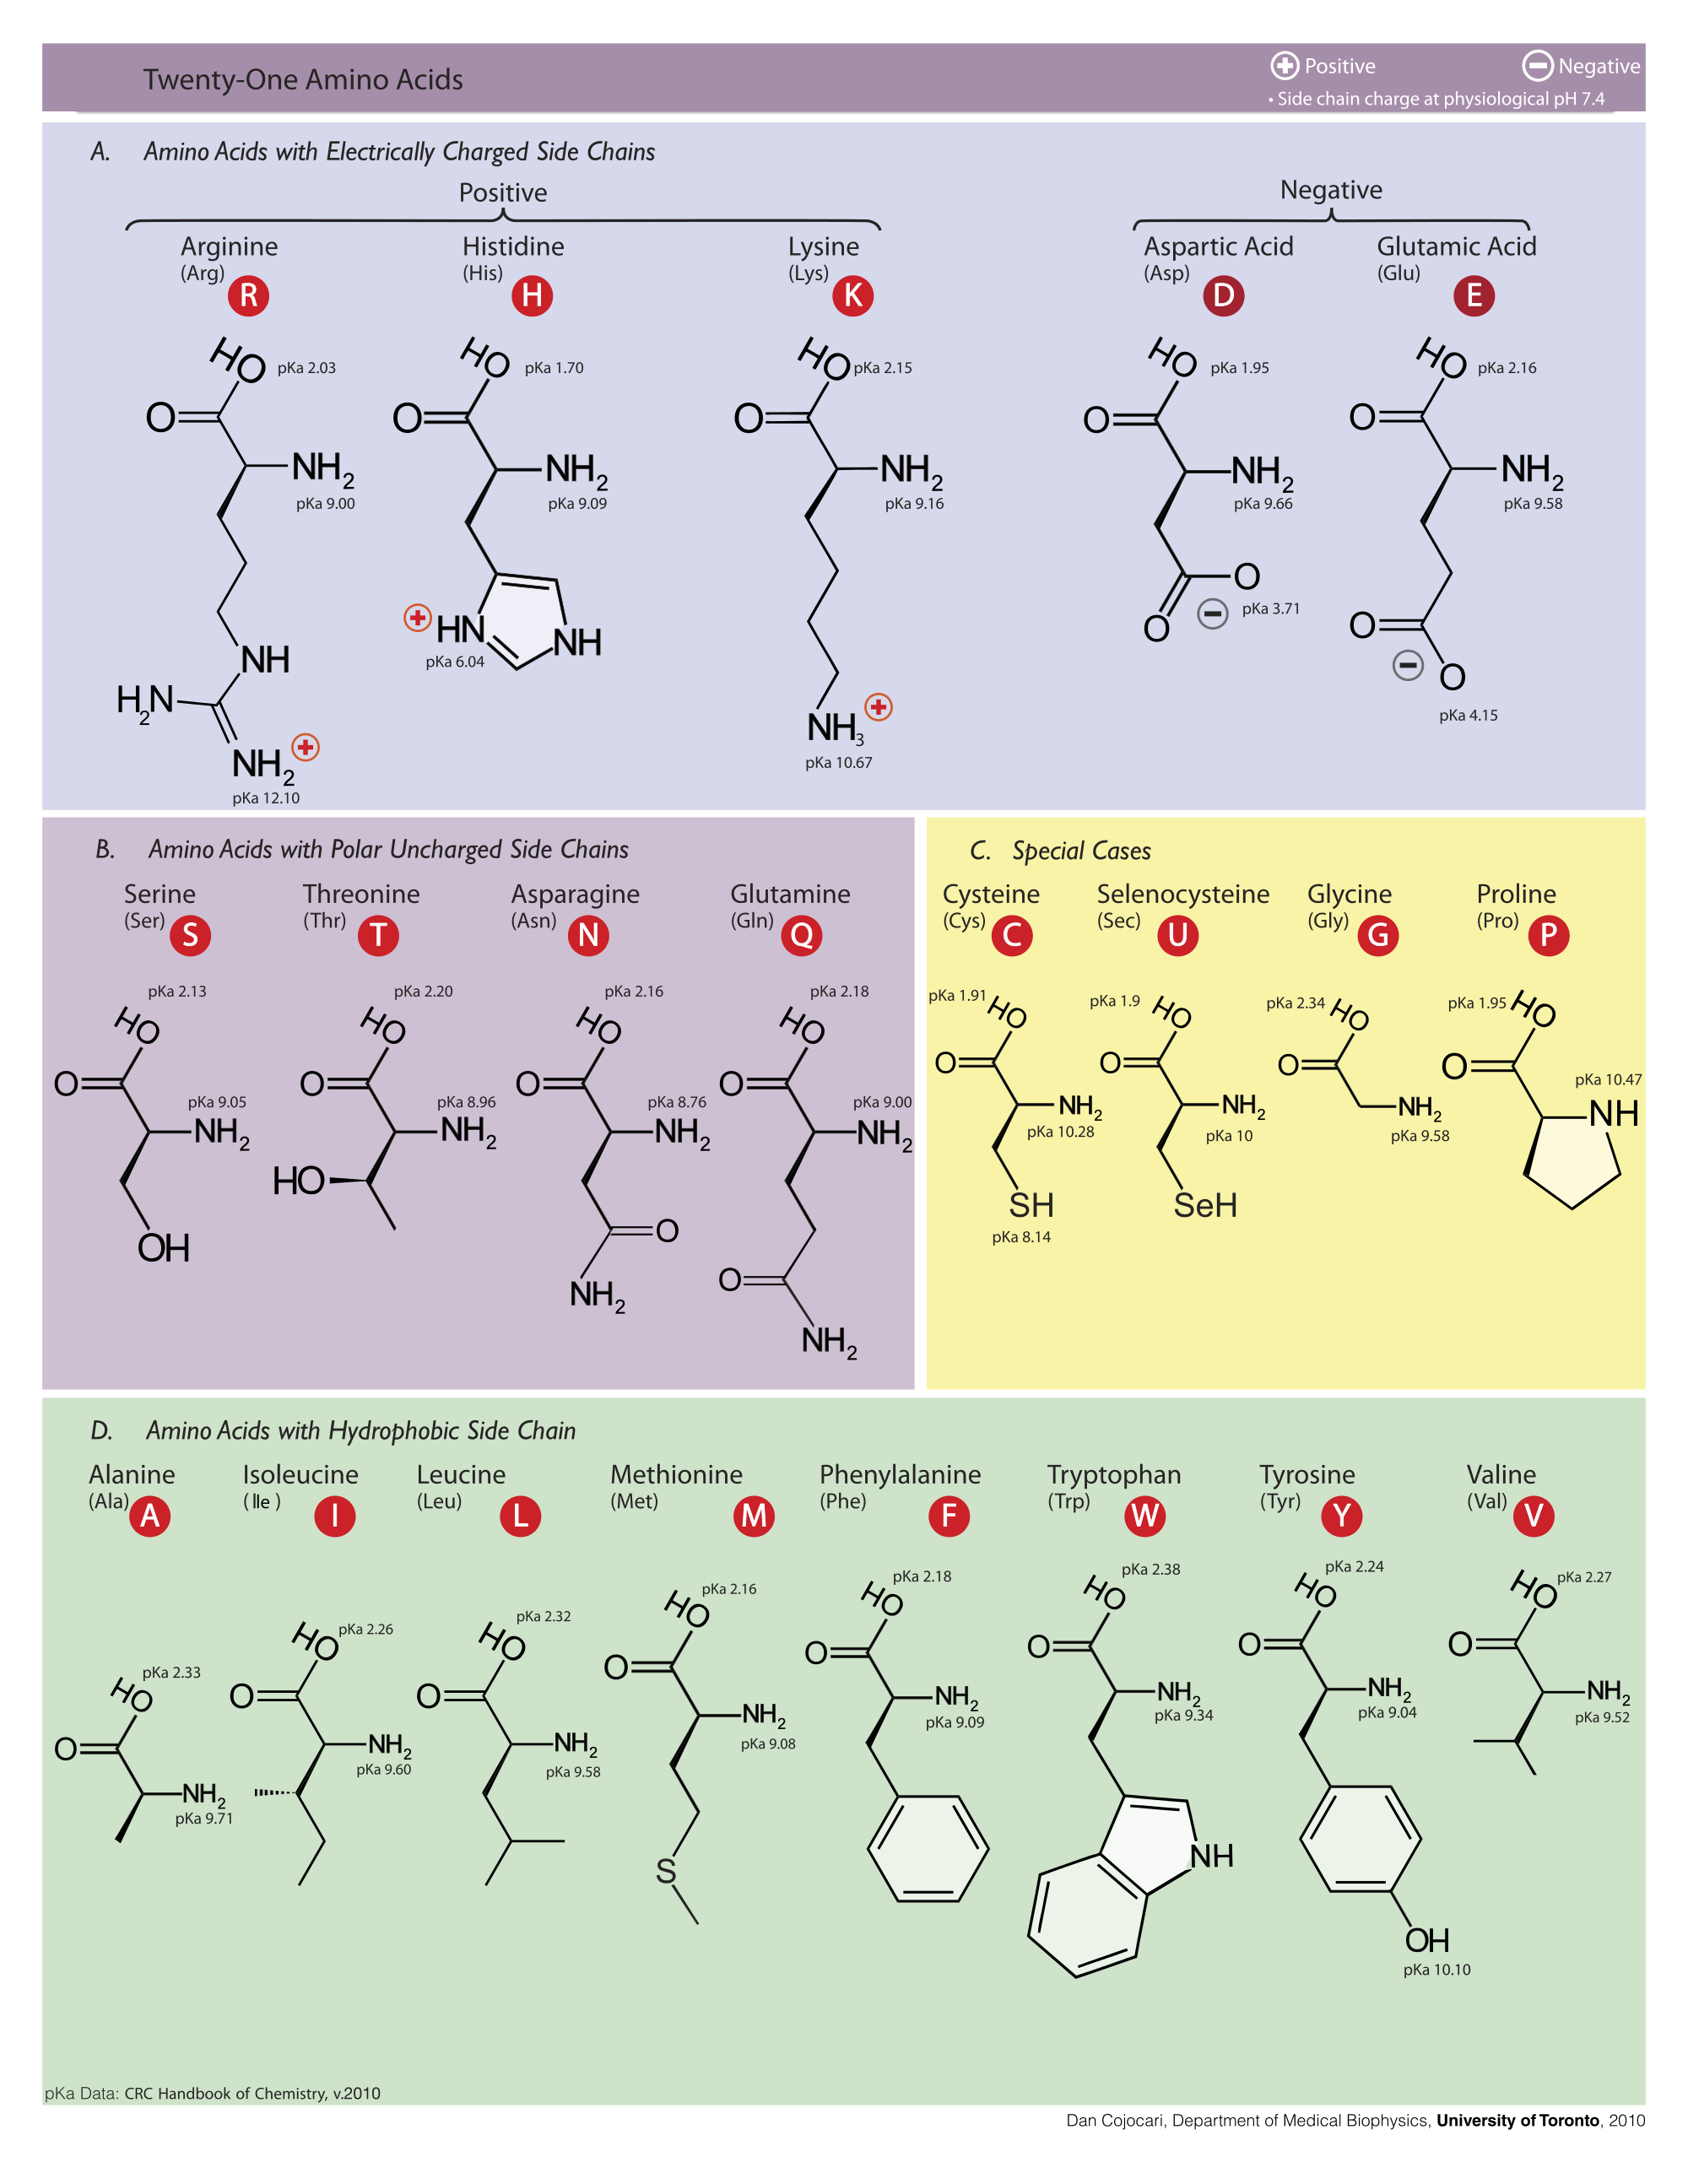
\includegraphics[width=0.8\textwidth]{Molecular_structures_of_the_21_proteinogenic_amino_acids.png}
	%\end{center}
	\caption{The 21 types of amino acid encoded in eukaryotic DNA, chategorized by their electrical properties. Full names, along with three letter and single letter abbreviations are given. Chemical structures are oriented so that the carboxyl group, $\alpha$-carbon, and amine groups are on top, with the side chain extending downwards.}
	\label{fig:aminoacids}
\end{figure}
%TODO: How to include liscence for this figure?

Two amino acids link together when the nitrogen atom from one's amine group bonds covalently with the carbon atom of another's carboxyl group, releasing a water molecule in the process.
This covalent bond is called a peptide bond, and an amino acid involved in at least one such bond is referred to as an \textit{amino acid residue}, or \textit{residue}.

A \textit{peptide}, or \textit{peptide chain}, is a linear chain of amino acids held together by peptide bonds, and the \textit{backbone} of the peptide consists of all atoms participating in peptide bonds, together with the $\alpha$-carbons.
If a peptide contains several residues it is referred to as a \textit{polypeptide}.
Proteins consist of one or more polypeptides which are bound together.
All peptides have a canonical ordering, from the \textit{N-terminus}, the residue with a free amine group, to the \textit{C-terminus}, the residue with a free carboxyl group.
This matches the order that polypeptides are created during biological protein synthesis.
Figure \ref{fig:3res} shows a ball and stick model of a small peptide.

\begin{figure}
	\centering
	%\begin{center}
	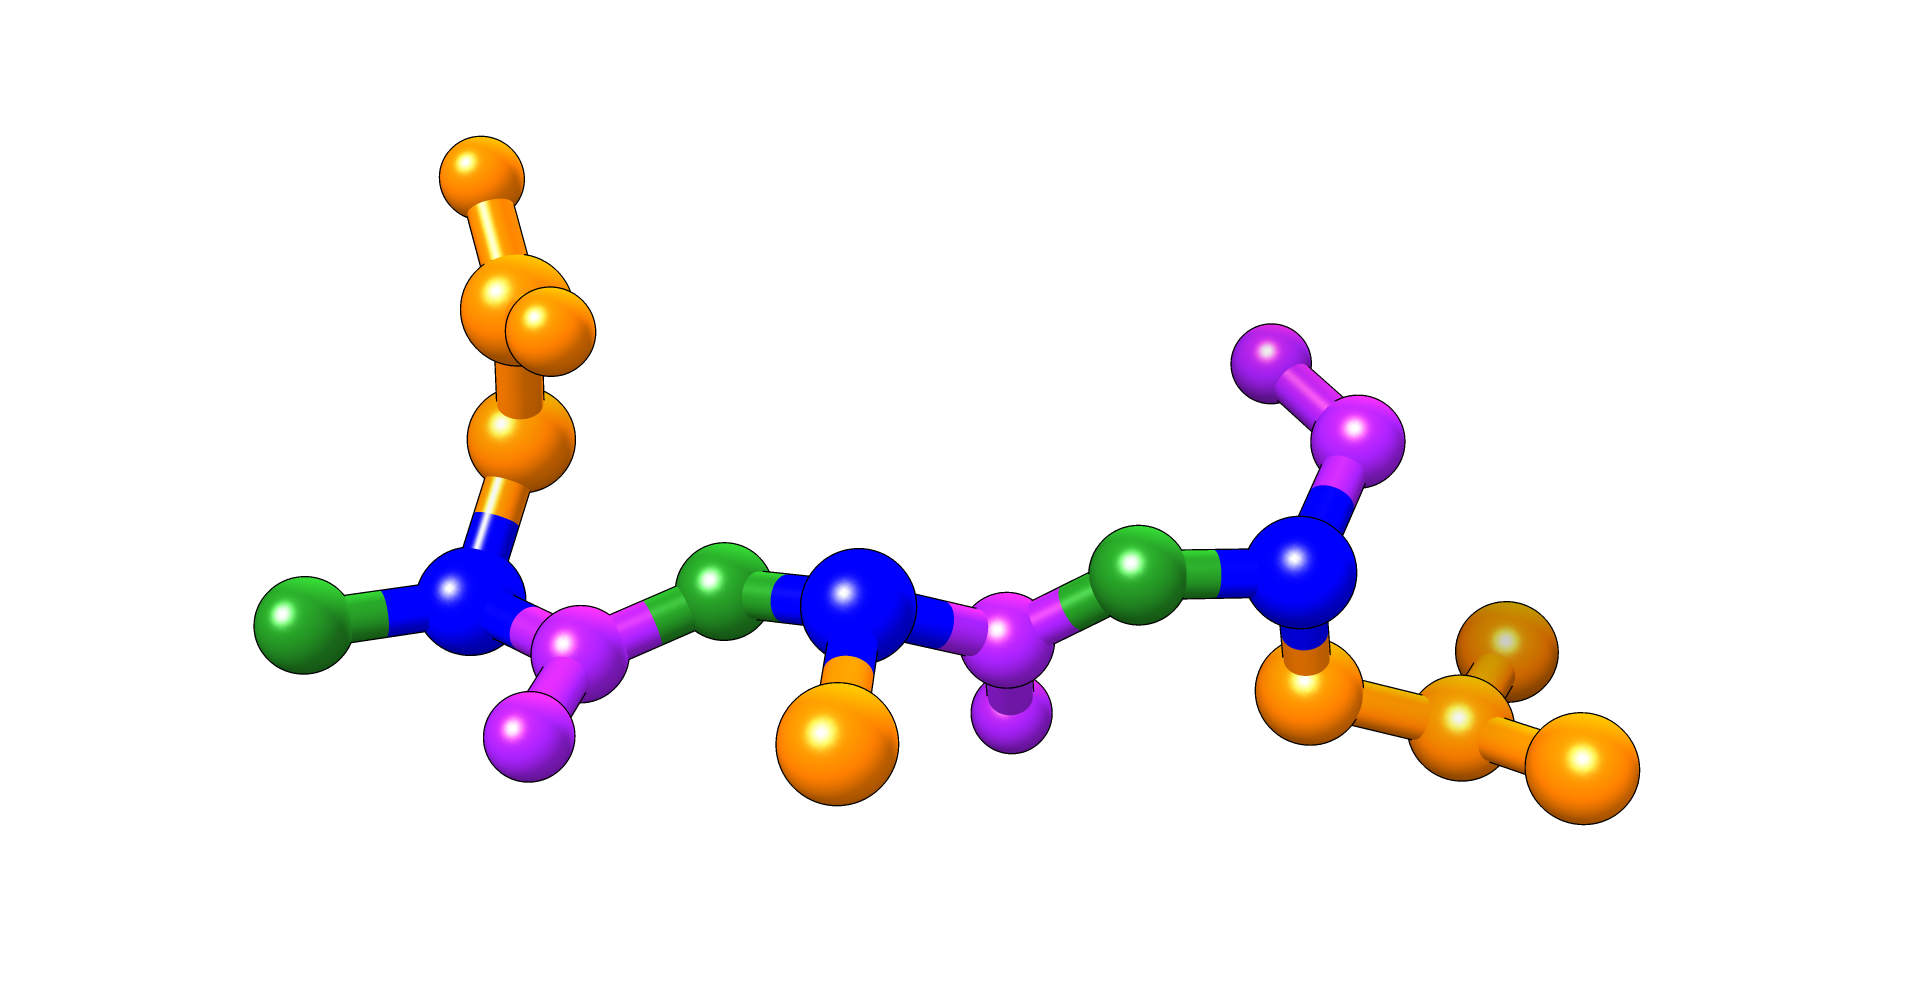
\includegraphics[width=0.8\textwidth]{1dab_3res_3x3.png}
	%\end{center}
	\caption{Ball and stick model of a peptide containing three amino acid residues (hydogens omitted). Colors indicate, blue: $\alpha$-carbon , orange: side chain, purple: carboxyl group after loss of OH, green: amine group after loss of H. Peptide bonds are between purple and green atoms. The backbone extends horizontally along blue, purple, and green atoms. Each sequence of atoms starting at an $\alpha$-carbon and ending at the next $\alpha$-carbon lay in an amide plane. From left to right are Aspartic Acid, Alanine, and Leucine. Created with Chimera~\cite{pettersen2004}.}
	\label{fig:3res}
\end{figure}

A residue's side chain influences how it interacts with other amino acids or other atoms and molecules. 
For example, oppositely charged side chains are be attracted to each other.
Polar side chains, being hydrophilic, are attracted to water molecules, and non-polar side chains, being hydrophobic, will prefer to avoid water and other polar molecules.
Such interactions play an important role in how proteins fold into 3D structures \cite{scheeffink2003}.

%TODO: mention globular proteins vs other kinds?


\subsection{Protein Structure}

Protein structure can be described via four levels of abstraction, termed \textit{primary}, \textit{secondary}, \textit{tertiary}, and \textit{quaternary} structure.
Primary structure refers to the sequence of amino acid residues (from N-terminus to C-terminus) in a single polypeptide, and is determined by the sequence of codons in the corresponding coding mRNA from which the protein is translated.
Sequences are typically written using a string of letters, where each unique letter corresponds to a different residue type. 

The physical chemistry associated with peptide bonds gives rise to the property that the nitrogen and carbon atoms involved in the peptide bond, along with the adjacent $\alpha$-carbons, all lie within a plane, called the \textit{amide plane}.
Each $\alpha$-carbon lies on the intersection between two amide planes, and the planes are free to rotate with respect to each other. 
%TODO: figure?
In some cases, side chains prohibit certain relative angles due to \textit{steric constraints}, which enforce that no two atoms may occupy the same volume of space at the same time.
In general, however, the angle between amide planes provides flexibility in the peptide backbone, which allows for the formation of higher order structures.

Secondary structure describes the local 3D structures that arise from the attraction of non-adjacent residues in a polypeptide.
There are three common categories of local structures: $\alpha$-helices, $\beta$-sheets, and loops.
An  $\alpha$-helix occurs when the polypeptide coils into a barrel-like structure (like the threads of a screw) and residues from adjacent coils (a distance of three residues from each other along the backbone) form hydrogen bonds with one another.
A $\beta$-sheet occurs when two non-adjacent sections of the polypeptide align next to each other such that residues in one of the sections form hydrogen bonds with residues in the other section.
$\beta$-sheets may be parallel or anti-parallel, depending on the relative orientation of adjacent strands in the sheet.
Figure \ref{fig:beta} illustrates the difference between parallel and anti-parallel $\beta$-sheets.
\begin{figure}
	\centering
	%\begin{center}
	\subfloat[Parallel $\beta$-sheets]{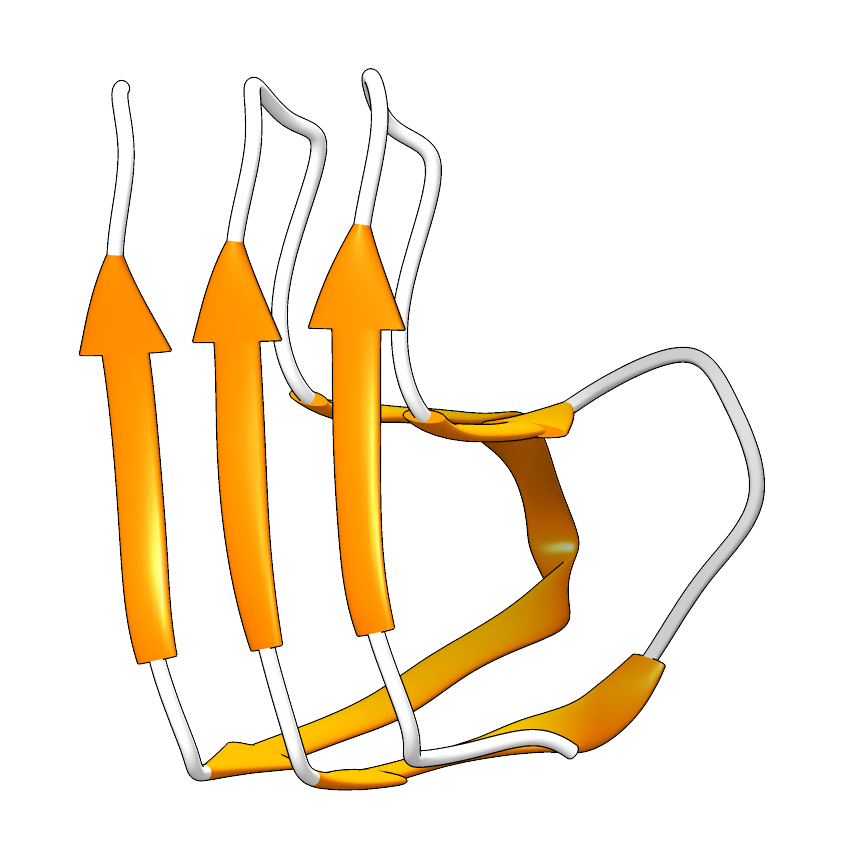
\includegraphics[width=0.4\textwidth]{1dab_end_betaP_3x3_cropped.png}\label{fig:beta_para}}
	\hfill
	\subfloat[Anti-parallel $\beta$-sheets]{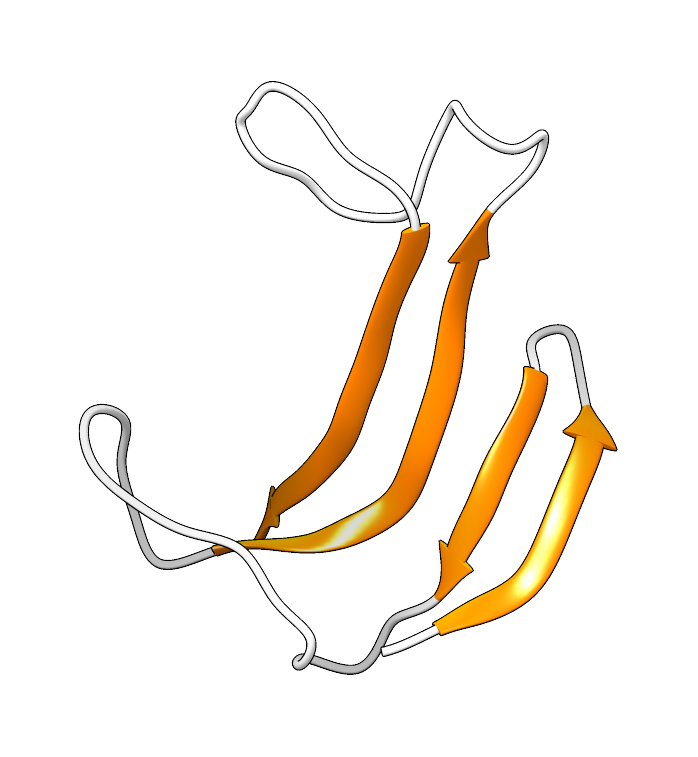
\includegraphics[width=0.4\textwidth]{1ca2_part_betaA_3x3_cropped.png}\label{fig:beta_anti}}
	%\end{center}
	\caption{Cartoon examples of parallel and anti-parallel $\beta$-sheets. In parallel $\beta$-sheets, adjacent strands in the sheet are oriented the same way, whereas in anti-parallel $\beta$-sheets, adjacent strands are oriented opposite each other. Created with Chimera~\cite{pettersen2004}.}
	\label{fig:beta}
\end{figure}
Some sections of the polypeptide form neither helices nor sheets, and are called loops.
These sections are more flexible than helices or sheets due the lack of hydrogen bonds, and therefore are useful in connecting the end of one helix/sheet to the beginning of another.
Figure \ref{fig:5nji_ss} shows a cartoon depiction of part of a protein, with different secondary structural elements highlighted in different colors.
	
\begin{figure}
	\centering
	%\begin{center}
	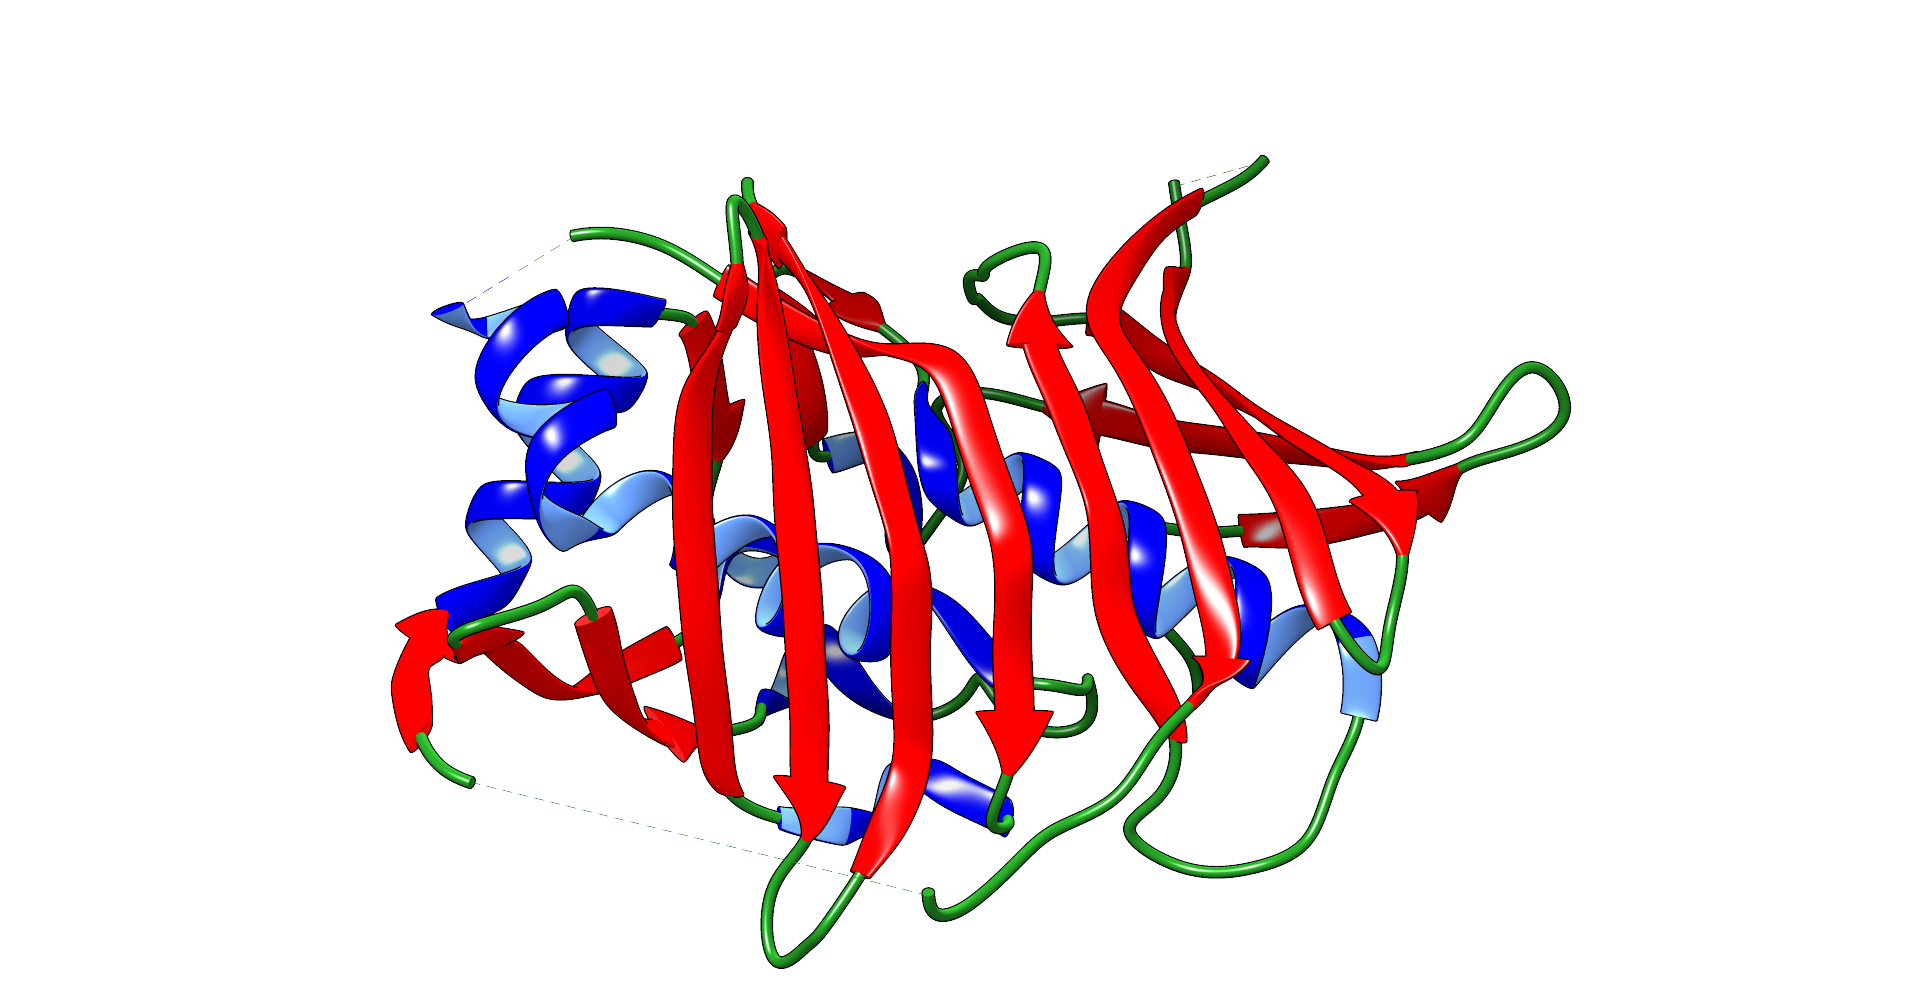
\includegraphics[width=0.8\textwidth]{5nji_ss_ch_3x3.png}
	%\end{center}
	\caption{3D cartoon of the the dehydratase domain of PpsC protein from Mycobacterium tuberculosis (PDB entry 5NJI~\cite{faille2017}) showing $\alpha$-helices in blue, $\beta$-sheets in red, and loops in green. Created with Chimera~\cite{pettersen2004}.}
	\label{fig:5nji_ss}
\end{figure}

Helices and sheets provide some rigidity to a polypeptide, but it typically further folds into a larger, tertiary structure, which may be globular, fibrous, or such that they reside on a cellular membrane.
After folding, some residues reside on the surface while others are buried in the core.
Because water makes up the majority of the cellular environment, protein surfaces have a higher percentage of hydrophilic residues than cores, and cores likewise have a higher percentage of hydrophobic residues than surfaces. 
Protein cores also show higher evolutionary conservation compared to surfaces~\cite{yan2008}.


Finally, in many cases multiple polypeptides combine together into a complex~\cite{scheeffink2003}.
%complexes may be \textit{obligate}, meaning they persist 
Quaternary structure describes the manner in which the individual polypeptides, known as subunits in this context, combine together to form the complex.
Protein complexes can be categorized as either \textit{transient} or \textit{permanent}.
This distinction reflects the difference in binding affinity (strength of attraction) between single proteins in the complex, with permanent complexes having higher and transient complexes having lower affinity.
Complexes can also be categorized as either \textit{obligate} and \textit{non-obligate}.
The constituent proteins of obligate complexes typically exist only in the complex, whereas for a non-obligate complex, each constituent protein exists both in the complex and independently.
Transience usually implies non-obligation and obligation usually implies permanence, so a simpler classification of obligate vs. transient is also appropriate~\cite{jones1996, perkins2010}.
The temporary nature of transient interactions enables complex networks of interaction which give rise to numerous cellular processes and the regulation thereof~\cite{perkins2010, ofran2003}.
Proteins in which all subunits are identical are called homomeric whereas proteins with different subunits are called heteromeric.
Homomeric proteins are usually obligate and more conserved than heteromeric proteins~\cite{jones1996}\cite{yan2008}

% receptor-ligand interaction and signal transduction.
% example of each: substrate-level phosphorylation, protein hormones, transcription factors, antibodies.


\subsection{Protein Interfaces And Their Prediction}

%TODO: mention ligand and receptor

The locus of a protein-protein interaction is the interface, which is comprised of pairs of residues, one from each interacting protein.
These pairs may form a disulfide bond or salt bridge which help anchor the two proteins together~\cite{yan2008}, but this is not always the case~\cite{ofran2003}.
Residues may not attract each other directly but still be considered part of the interface due to their proximity.
This is the case when hydrophobic residues from two proteins appear near each other in the interface, since they do not attract each other, but this configuration is energetically favorable compared to being exposed to water in the surrounding cellular environment~\cite{yan2008, ofran2003}.
Historically, residues have been considered part of the interface if they are in contact with residues on the adjacent protein. 
This is typically determined in one of two ways, either the distance between any atom in the residue in question and any atom in the other protein is below a threshold, or the exposed area of a residue drops sufficiently after complex formation. ~\cite{yan2008, jones1996, ofran2003, minhas2014}.

A survey of known protein complex structures from the Research Collaboratory for Structural Bioinformatics (RCSB) Protein Data Bank (PDB)~\cite{berman2000} has shown that interfaces have a higher prevalence of hydrophobic residues, lower prevalence of hydrophilic residues, and more evolutionary conservation compared to non-interface surface regions~\cite{yan2008}.
The higher overall hydrophobicity of an interface region biases the protein towards configurations in which the interface excludes water by binding to another protein.
The higher degree of conservation shows the functional significance of the interfaces, although conservation is somewhat lower for transient compared to obligate complexes~\cite{jones1996}.
Transient complexes also have a comparatively~\textit{lower} hydrophobicity compared obligate complexes, consistent with the fact that proteins in transient complexes exist outside of the complex, with interfaces exposed to water~\cite{jones1996}.
To overcome the unfavorable energetic effects of burying more hydrophilic residues in an interface, transient interfaces also have relatively higher numbers of hydrogen bonds~\cite{jones1996}.
It has also been shown that transient complexes have less shape complementarity between the participating proteins compared to obligate complexes~\cite{jones1996}.
Lastly, transient interfaces also tend to either be smaller in size (for weakly interacting complexes)~\cite{jones1996, perkins2010}, or undergo more conformational change when forming (for strongly interacting complexes)~\cite{perkins2010} compared to obligate complexes.
These differences make transient complexes more difficult to distinguish from non-interface surface residues~\cite{perkins2010}.

Historically, the problem of interface prediction has been formulated in two ways: \textit{partner-independent} and \textit{partner-specific} prediction.
The former variant considers a single residue from a protein and attempts to answer the question: does this residue form part of the interface with some other partner protein?
The latter variant considers pairs of residues, each from a different protein, and attempts to answer a more specific question: does this \textit{pair} of residues constitute part of the interface between these two proteins?
The pairwise nature of partner-specific prediction allows the consideration of the compatibility of a pair of residues, which has been found to increase performance~\cite{ahmad2011, minhas2014}.
Methods of interface prediction include \textit{docking methods}, \textit{template-based methods}, and \textit{machine learning methods}.

Docking methods predict the 3D bound formation of two proteins in a complex, from which the interface can be extracted. 
These methods use energy minimization techniques~\cite{chen2003, zundert2016}.
Unlike template and machine learning methods, docking methods do not require a library of known interfaces in order to make predictions, but are historically poor at accounting for conformational change during complex formation~\cite{ezkurdia2009}.

Template based methods make predictions based on similar known interfaces.
The protein of interest is compared to a library of interfaces, and the interface is predicted from the most similar interfaces from the library.
Template methods rely on a non-redundant library and can make predictions only when there is a sufficiently close match to an interface in the library~\cite{tuncbag2011}.

Machine learning methods attempt to directly predict the interface rather than comparing against a template complex or predicting the bound formation, however they still use information from a library of complexes whose interfaces are known.
Machine learning approaches have included use of neural networks and support vector machine~\cite{ahmad2011}~\cite{minhas2014}.
The latest SVM based approach, PArtner-specific Interacting Residue PREDictor (PAIRpred), uses pairwise kernels which operate on pairs of residues and incorporates both sequence and structural information of residues.
The method performs well compared to existing docking and machine learning methods~\cite{minhas2014}. More detail of prior work in interface prediction will be given in Chapter \ref{chap:relatedwork}.